\documentclass[journal,12pt,twocolumn]{IEEEtran}
\usepackage{amsmath,amssymb,amsfonts,amsthm}
\usepackage{txfonts}
\usepackage{tkz-euclide}
\usepackage{listings}
\usepackage{gvv}
\usepackage[latin1]{inputenc}
\usepackage{adjustbox}
\usepackage{array}
\usepackage{tabularx}
\usepackage{enumitem}
\usepackage{pgf}
\usepackage{lmodern}
\usepackage{circuitikz}
\usepackage{tikz}
\usepackage{graphicx}


\begin{document}
\bibliographystyle{IEEEtran}

\vspace{3cm}

\title{}
\author{EE23BTECH11054 -  Sai Krishna Shanigarapu$^{*}$
}
\maketitle
\newpage
\bigskip

% \renewcommand{\thefigure}{\theenumi}
% \renewcommand{\thetable}{\theenumi}

\section*{Gate EE 2023}
54. \hspace{2pt}In a circuit, there is a series connection of an ideal resistor and an ideal capacitor.
The conduction current (in Amperes) through the resistor is $2\sin\brak{t + \frac{\pi}{2}}$. The displacement current (in Amperes) through the capacitor is \rule{1cm}{0.15mm}.\\ 
\begin{enumerate}[label=(\Alph*)]
    \item $2\sin\brak{t}$
    \item $2\sin\brak{t+\pi}$
    \item $2\sin\brak{t +\frac{\pi}{2}}$
    \item $0$
\end{enumerate}
\hfill(GATE EC 2022)

\solution

\begin{table}[ht]
     \begin{adjustbox}{width=\columnwidth}
       \setlength{\arrayrulewidth}{0.3mm}
\setlength{\tabcolsep}{20pt}
\renewcommand{\arraystretch}{1.5}

\begin{tabular}{|c|c|c|}
\hline
Parameter& Description & Value\\
\hline
$I_c$ & Conduction Current & $2\sin\brak{t + \frac{\pi}{2}}$\\
\hline
%$I_d$ & Displacement current & ?\\
%\hline
$A$ & Cross-sectional area & \\
\hline
\end{tabular}

    \end{adjustbox}
    \caption{Parameters}
    \label{tab:tab_gate_ec_2022_24_1}
\end{table}

\begin{figure}[ht]
  \centering
      \begin{circuitikz}[american]
\draw (0,3) to [short,*-, i=$i_c$] (1,3) to [R=$R$] (4,3);
\draw (0,0) to [short, *-] (4,0);
\draw (4,3) to [short, i=$i_d$] (4,2.5) to [C=$C$] (4,0);
\end{circuitikz}
  \caption{Circuit 1}
\end{figure}

From Table \ref{tab:tab_gate_ec_2022_24_1}
\begin{align}
    J &= \overline{J_c} + \overline{J_d}
\end{align}
%\newpage



\begin{figure}[ht]
  \centering
      \begin{tikzpicture}

        \draw[->] (-0.5,0) -- (4.5,0) node[right]{$E_{\text{ref}}$};
        \draw[->] (0,-0.5) -- (0,4.5) node[above]{$J_d$};
        

        \draw (0,0) -- (4,4);
        

        \draw[dashed] (4,0) -- (4,4);
        \node[right] at (4,4) {$\overline{J}$};
        \draw[dotted] (4,4) -- (4,0) node[below]{$J_c$};

        \draw[dashed] (0,4) -- (4,4);
        \draw[dotted] (4,4) -- (0,4) node[left]{$J_d$};
        

        \draw[->] (0.5,0) arc (0:90:0.5);
        \node[right] at (0.5,0.3) {$\frac{\pi}{2}$};
\end{tikzpicture}


  \caption{Phasor plot}
\end{figure}
From figure \ref{fig:fig_gate_ec_2022_24_1},\\
$\overline{J_d}$ leads $\overline{J_c}$ by $\frac{\pi}{2}$ $\implies$  $i_d$ leads $i_c$ by $\frac{\pi}{2}$\\

Hence,
\begin{align}
    i_d &= 2\sin\brak{t + \frac{\pi}{2} + \frac{\pi}{2}}\\
    \implies i_d &= 2\sin\brak{t+\pi}
\end{align}

$\therefore$ (B) is correct.

\begin{figure}[ht]
    \centering
    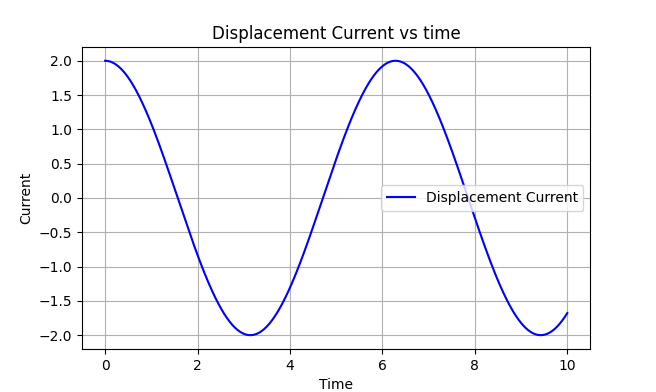
\includegraphics[width=\columnwidth]{figs/Figure_1.png}
    \caption{Plot of $i_c$ and $i_d$ vs time}
    \label{fig:fig_gate_ec_2022_24_1}
\end{figure}



\end{document}
